\documentclass[../main.tex]{subfiles}
\graphicspath{{assets/}{../assets/}}

\usepackage{multirow}

\begin{document}

    \section{Prévision d'organisation du projet}


    \paragraph{}
    Le code source de l’application sera disponible sur Github à l’adresse suivante: \url{https://github.com/Guillaume-prog/projet-fil-rouge}

    \paragraph{}
    Au sein de l’équipe, des outils de gestion comme Trello vont être utilisés.

    \subsection{Déroulement prévu}

    \paragraph{}
    Voici une planification prévisionnelle du projet sous la forme d’un diagramme de Gantt réalisé avec Gantt Project:

    \begin{figure}[H]
        \centering
        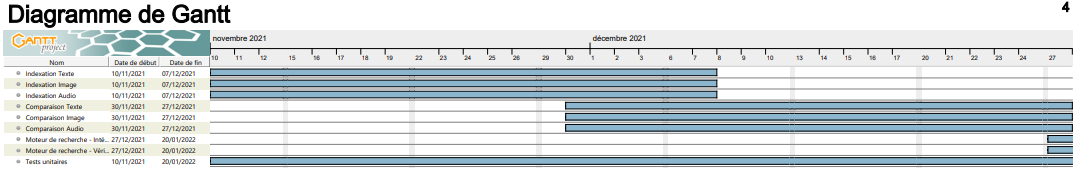
\includegraphics[width=160mm]{gantt/gantt_calendar.png}
        \caption{Diagramme de Gantt du projet}
    \end{figure}

    \begin{figure}[H]
        \centering
        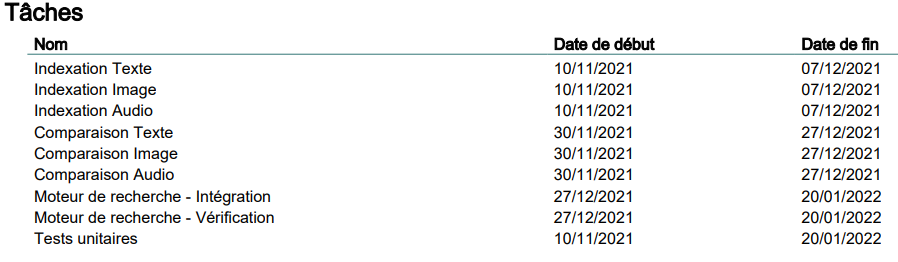
\includegraphics[width=160mm]{gantt/gantt_list.png}
        \caption{Tableau récapitulatif des tâches à réaliser issu du diagramme de Gantt}
    \end{figure}

    \subsection{Répartition des tâches}

    \begin{table}[H]
        \centering
        \begin{tabular}{ | m{10em} | m{10em} | m{10em} | }
            \hline
            \rowcolor{Gray} Tâches & Sous-tâches & Affectation des tâches \\
            \hline
            \multirow{3}{10em}{Indexation} 
            & Indexation texte & Guillaume \& Peter \\
            \cline{2-3}
            & Indexation image & Constant \& Peter \\
            \cline{2-3}
            & Indexation audio & Julian \& Nelson \\
            \hline

            \multirow{3}{10em}{Comparaison} 
            & Comparaison texte & Guillaume \& Constant \\
            \cline{2-3}
            & Comparaison image & Constant \& Peter \\
            \cline{2-3}
            & Comparaison audio & Julian \& Nelson \\
            \hline

            \multirow{2}{10em}{Moteur de recherche} 
            & Intégration & Toute l'équipe \\
            \cline{2-3}
            & Vérifications & Julian \& Nelson \\
            \hline

            \multirow{1}{10em}{Test} & / & Toute l'équipe \\
            \hline


            \hline
        \end{tabular}
        \caption{Récapitulatif des affectations des tâches du projet}
    \end{table}

\end{document}